\subsubsection{Data Access Layer}
Data Access Layer består af tre dele. Den første del består i at modtage en produktoversigt fra CentralServer. Den anden del består i at sende information om gennemførte køb til CentralServer. Den tredje del består i at denne salgskvitteringer efter køb er gennemført.

\begin{figure}[H]
	\centering
	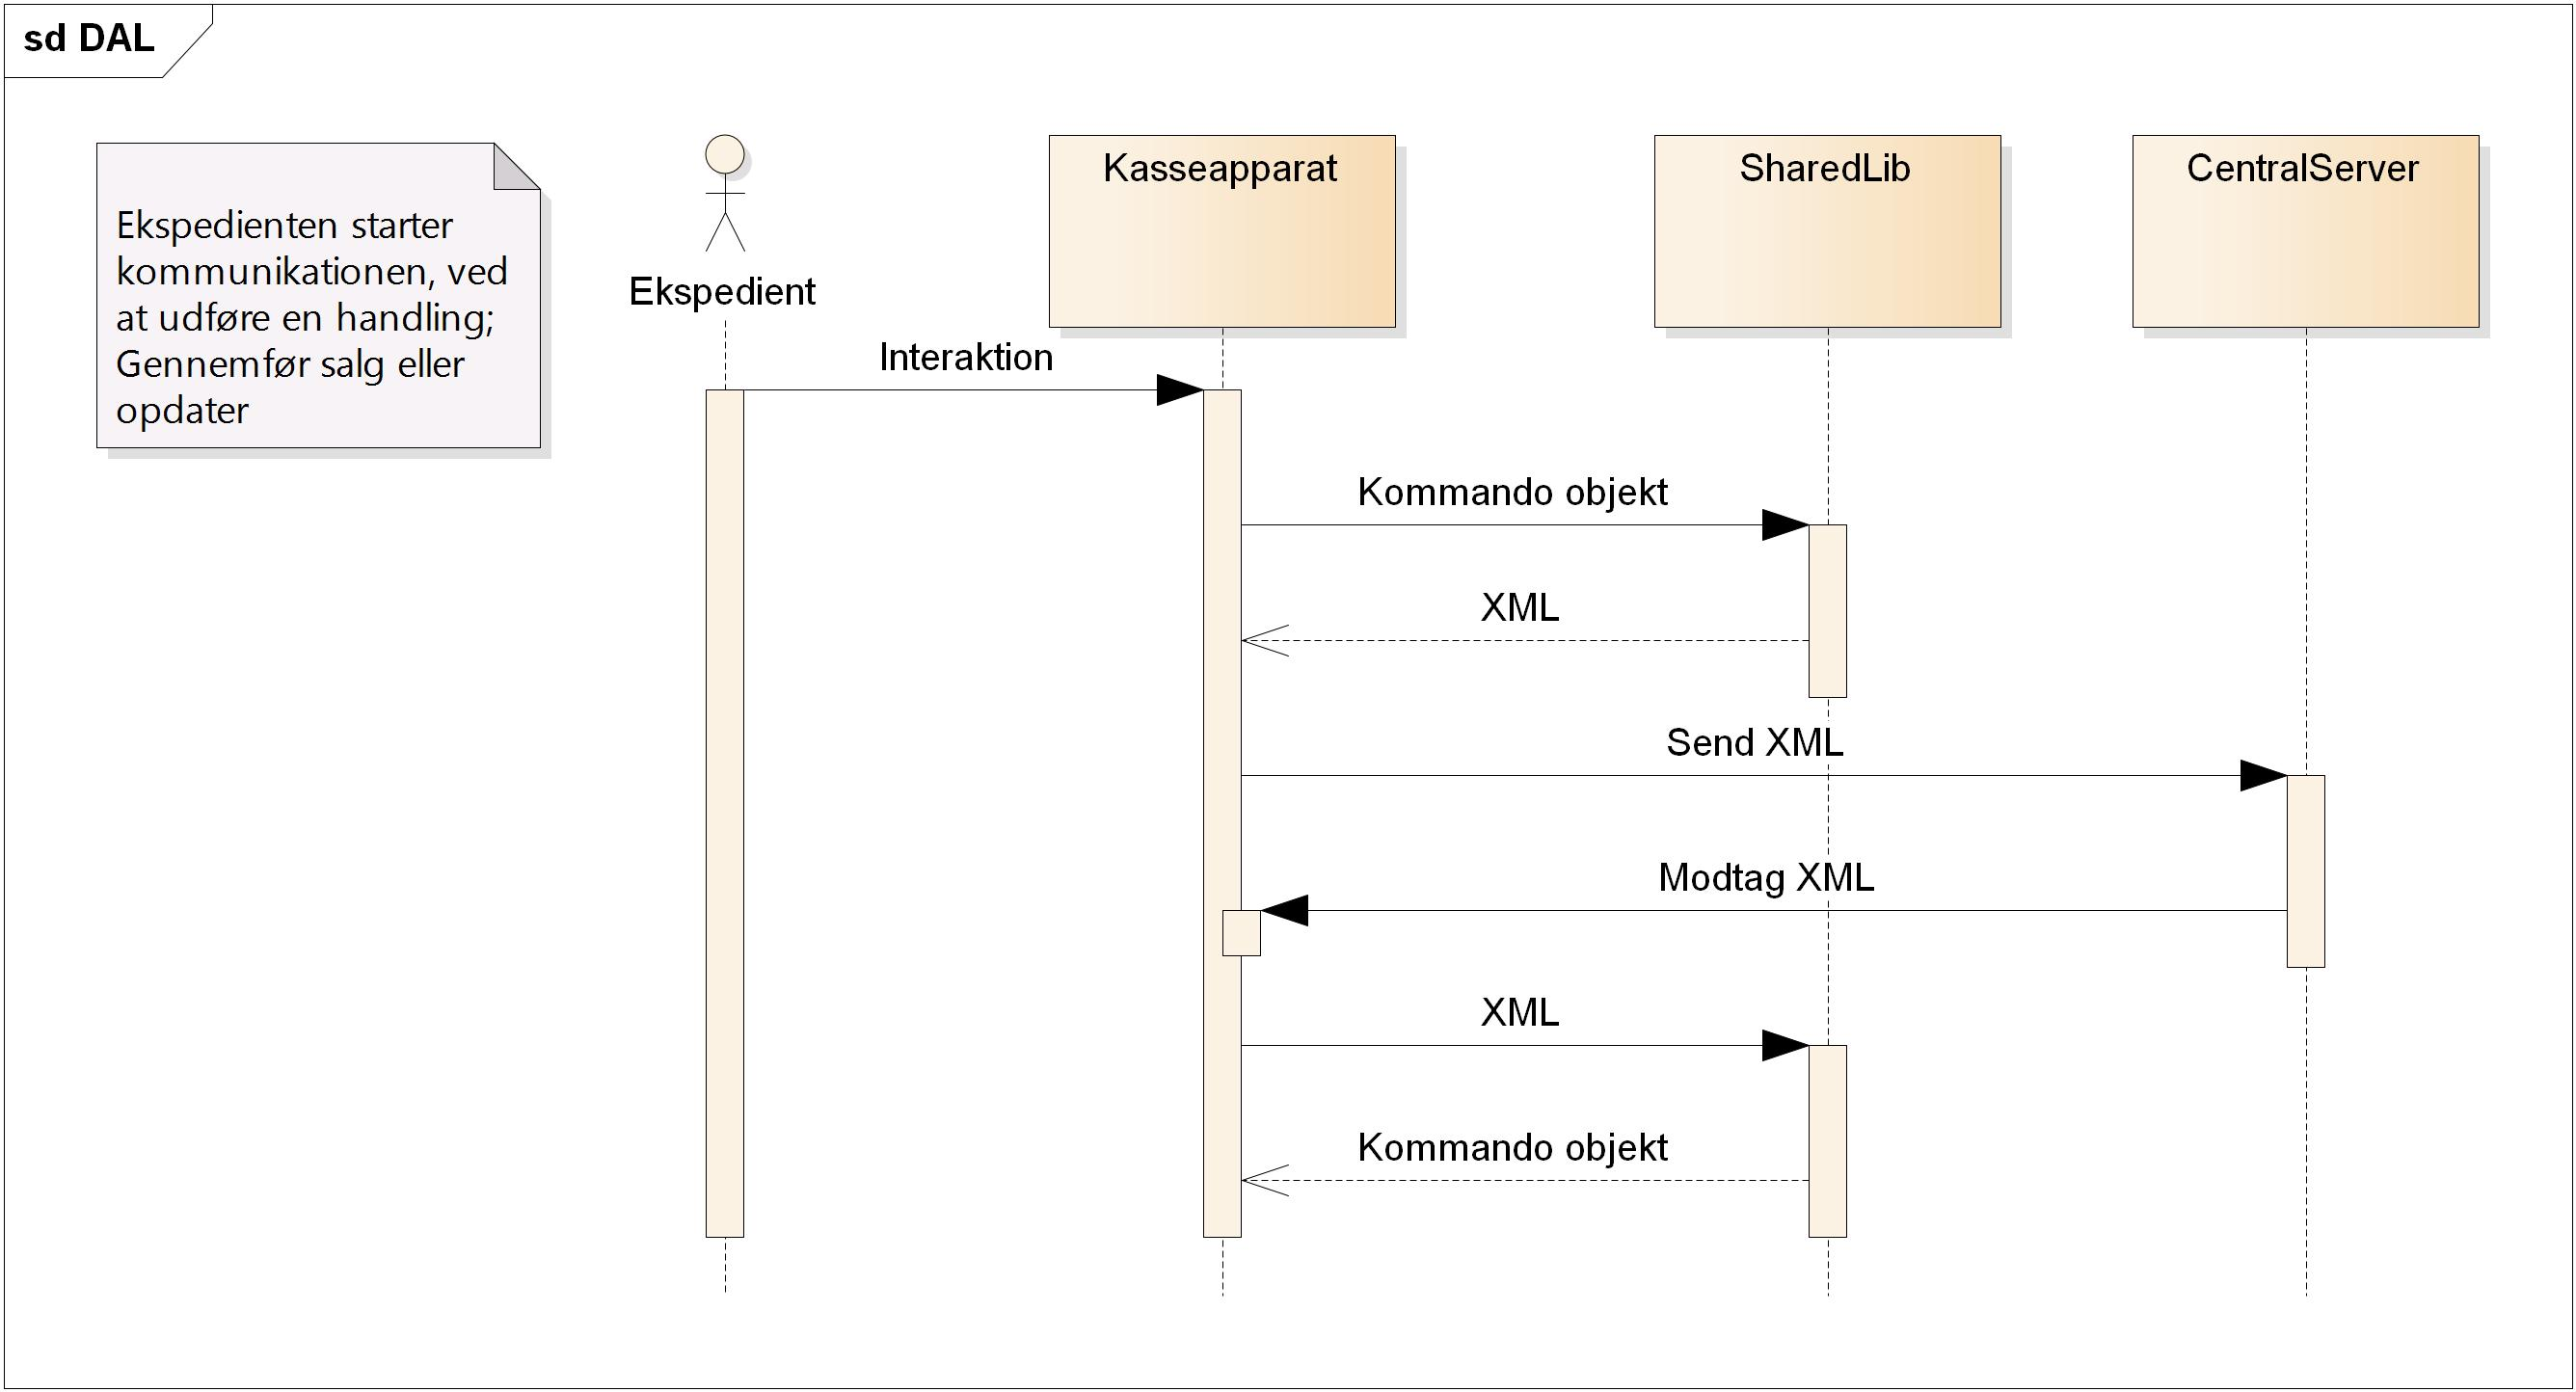
\includegraphics[width=\textwidth]{Projektbeskrivelse/DesignOgImplementering/Frontend/Pics/DALsq}
	\caption{Kommunikation til/fra CentralServer}
	\label{fig:KAtCS}
\end{figure}

Figur \ref{fig:KAtCS} viser et generelt eksempel på hvordan kommunikationen til CentralServer fungerer. Ekspedient gennemfører f.eks. et køb i brugergrænsefladen, herefter laves et kommando objekt, som encodes til en XML-streng ved hjælp af SharedLib. Denne XML string sendes til CentralServer. Forventes et svar modtages dette i form af en XML string, denne decodes til et kommando objekt, som indeholder informationen.\\
Oprettelse af salgskvitteringer foregår ved at der oprettes en tekstfil, navngivet efter tidspunkt for købet.
